\chapter{Lattice gass cellular automata}
The first lattice gass cellular automaton was proposed in 1973 by Hardy, Pomeau and de Pazis, hence it is generally known as HPP model.

Unfortunately, it could not do its job sufficiently well. For the reasons that we will explore in this chapter, its macroscopic limit does not converge to Navier-Stokes equations.

\bigskip

In the subsequent chapters we will explore two different approaches how to make functional LGCA. They both build on the idea this imperfect HPP.

Therefore, it is worthwhile to explain the basic principles of HPP first, and later on, we will upgrade it - either to FHP, Pair-interaction or their multi-dimensional variants.

\section{From CA to LGCA}

Lattice of HPP is the simple rectangular 2D grid. At every point of a grid, there is node sitting in, and this node is composed of 4 cells, see Figure~\ref{rectangular}.

\begin{figure}[htbp]
 \centering
 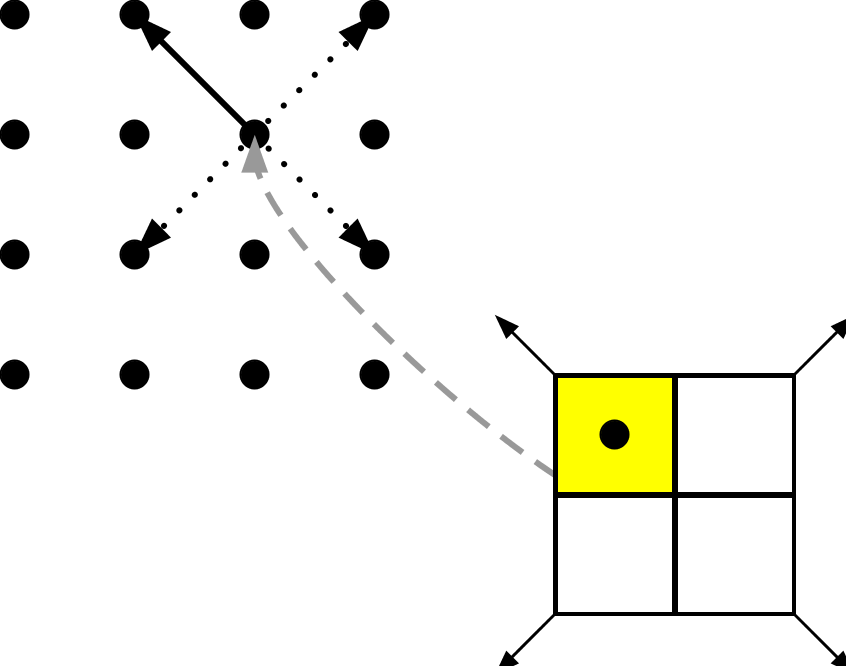
\includegraphics[width=0.6\textwidth]{./img/hpp}
 \label{rectangular}
 \caption{Rectangular grid}
\end{figure}

Each cell of the node can be in two states -- empty (white square) or occupied by the particle (yellow square on the figure \ref{rectangular}).
The particles are heading to the diagonal nodes.

\section{Update rule}
The update rule should be design in such a manner, that is conserve physically relevant quantities, namely mass and momentum.

So far we have the grid full of particles.
For any LGCA model, update is done in two subsequent steps -- collision and propagation.

In the collision step, In HPP, there are only two collision configurations, and one collision rule that guides them, see Figure~\ref{hpp-colision}.

\begin{figure}
 \centering
 \includegraphics[width=0.6\textwidth]{./img/hpp_col}
 \label{hpp-colision}
 \caption{HPP colisions}
\end{figure}

We see this configurations are symmetric. The first configuration is resolved to the other and vice versa.

It is easy to understand that there are no other collision configurations and collision rules. If any other state gets changed, it would break the conservation of momentum and would be physically unrealistic.

\section{Propagation:}

After the collision is resolved, propagation follows.
During propagation, particle from the upper-left cell moves to the upper-left node, and will occupy they same cell (with the same velocity vector), so that momentum is also conserved by the propagation.

\begin{figure} [h]
 \centering
 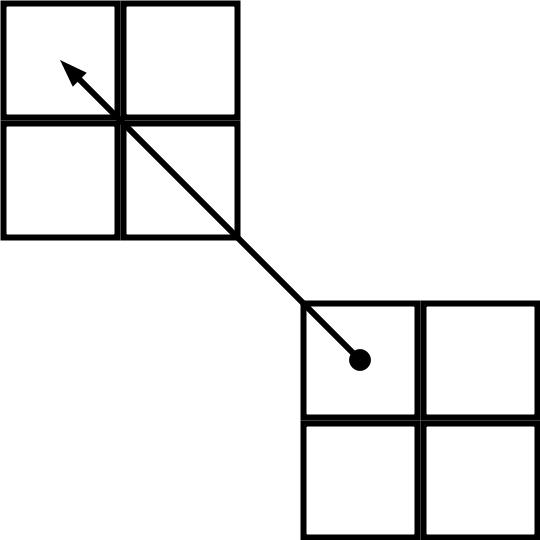
\includegraphics[width=0.3\textwidth]{./img/propleft}
 \label{hpp-colision}
 \caption{Propagation of particle from upper-left cell}
\end{figure}

\bigskip

\section{Conservation laws}

We already noted that collision and propagation conserve momentum, and they obviously conserve mass, since particles are neither created, nor anihilated in these processes. 
Let us inspect these conservation laws in the more depth by considering symmetries of this model.

Suppose we are using periodic boundary condition. Then, the finite rectangular grid of HPP is actually a torus. It is easy to imagine that if we shift the grid by the discrete step (of length 1), we get the very same torus.
So this rectangular grid of HPP is symmetric with respect to translation.
As we know by Norther's theorems, translational symmetry implies conservation of momentum.

\bigskip

Also, the grid possesses some rough rotational symmetry - rotating the grid by 90 degrees, we get the same grid.

However, this rotation by 90 degrees is too crude, and so HPP do not preserve the angular momentum. This is the flaw of the model that cannot be overlooked - HPP do not preserve all physical quantities that Navier-Stokes equation would suggest.

Its another flaw goes in the opposite direction. HPP preserves quantities that are non-physical - so called spurious invariant.

Consider orientation of particles in Fig.\ref{hpp-colision} before colission.
One particle heads to north-east, the other south-west.
After the collision, one particle heads to north-west, other particle to south-east.
So the number of particles heading to the south, east, north and west do not change by collision (and neither by propagation). It is invariant as the time goes by.

To assert it more formally, let us decompose the total momentum into the cardinal directions:
\begin{align} 
P = P_N + P_S + P_E + P_W.
\end{align}
This total momentum $P$ is correctly conserved by HPP, but also quantities
\begin{align} \label{zanet}
P_{spur1} = P_N + P_E - P_S - P_W
\end{align}
and
\begin{align}
P_{spur2} = P_N + P_W - P_S - P_E
\end{align}
are conserved, although these quantities have no physical counterparts.

\bigskip

To conclude this chapter and finish-off the HPP, it is physically implausible because
\begin{enumerate}
\item angular momentum is not conserved due to insufficient rotational symmetry,
\item other non-physical quantities, so called \textit{spurious invariants} are conserved.
\end{enumerate}

Although it is flawed model, it sparked interest of the wider community and various successful LGCAs evolved from HPP. In the next chapter, we will introduce the first physically relevant branch of LGCAs -- the FHP model.